% 原文 pp.29–34（印刷 pp.1147–1152）
\section{Lecture 2：规范对称性破缺与红外行为续论}

\begin{keytakeaways}
本讲从哈密顿途径重新刻画规范场论：位形空间取为运动方程解空间 $\widetilde{M}_0$，物理相空间是辛商 $M=M_0/\!/\widehat{G}_0$，而真正被谈论"破缺"的对称群是无穷远处的常值规范变换群 $G_\infty=\widehat{G}/\widehat{G}_0$。核心数学工具是矩映射 $\mu:M_0\to\widetilde{\mathfrak g}_0^*$ 及其给出的哈密顿量 $Q(\varepsilon)$；用 Noether 形式与 Gauss 约束把 $Q(\varepsilon)$ 化为无穷远处球面上的通量积分，这说明"荷"是由边界（红外）数据决定的。以带复标量的 $U(1)$ 规范场论为例，作者区分了 $v^2>0$（唯一真空、无质量矢量加两个有质量标量）与 $v^2<0$（极小圆、Higgs 机制、全部场有质量）两种情形，并强调规范对称性破缺与整体对称性破缺有本质区别：极小圆上各点彼此规范等价，故只对应一个真空。最后把整体对称性与规范对称性联系起来：若物质拉氏量红外地自由，则"整体对称性破缺"与"规范化后出现 Higgs 机制"互为充要，并开启关于"不存在更高自旋无质量粒子"的一般性讨论。
\end{keytakeaways}

% ===== 原文 p.29 =====
% 原文 §2.1
%（原文标题页：LECTURE 2 / Gauge Symmetry Breaking and More on Infrared Behavior，印刷 p.1147。）
本讲的标题是 \emph{Gauge Symmetry Breaking and More on Infrared Behavior}（规范对称性破缺与红外行为续论）。

\subsection{规范对称性}

回顾规范对称性是什么。我们有时空 $X=\mathbb{R}_{\text{time}}\times X_0$。我们有一个紧致规范群（compact gauge group）$G$。我们有一个场论，其中的场位形（field configuration）是 $\mathbb{R}^d$ 上某个主丛（principal bundle）中的联络（connection），此外还可能有某些物质场（matter fields）。

回顾规范场论的哈密顿途径（Hamiltonian approach）。设 $\widetilde{M}_0$ 为经典运动方程的解所构成的空间。在 $\widetilde{M}_0$ 上有规范变换群 $\widehat{G}$ 的作用。设 $M_0\subset\widetilde{M}_0$ 为满足下述条件的全部解构成的空间：$G$-丛在时间方向上被平凡化，并且联络在该方向上为平凡。这类解一如往常完全由 $A(t_0)$、$\frac{dA}{dt}(t_0)$ 这一对数据（其中 $t=t_0$ 是一个空间切片）连同物质场的初始数据所决定。显然（It is clear that），$\widetilde{M}_0$ 的任一元素都可以借规范变换化到 $M_0$ 中，因此 $M_0$ 在规范变换的意义下仍然包含全部解。

% [Tutor Note: 作者说"显然"，实则用到两件事：(i) 时空取乘积形式 $X=\mathbb{R}_{\text{time}}\times X_0$，时间方向可缩，故任何主丛沿时间方向可平凡化；(ii) 丛平凡化后，沿 $t$ 解常微分方程 $\frac{dg}{dt}g^{-1}=-A_t$ 即可把 $A_t$ 规范掉。若时空不是乘积（例如含非平凡的时间方向缠绕），这一步不成立，$M_0$ 便不能捕获全部解。]

设 $X_0=\mathbb{R}^{d-1}$。此时我们可以只考虑平凡丛，并且（若能量有限）只考虑在空间无穷远处为平凡的联络。换言之，若 $\mathcal{A}$ 是 $\mathbb{R}^{d-1}$ 上平凡 $G$-丛的、在 $\infty$ 处为平凡的联络 $A$ 所构成的空间，则纯规范场论的 $M_0$ 就是 $T^*\mathcal{A}$。若存在物质场，则 $M_0$ 是 $T^*\mathcal{A}$ 与某个别的空间的乘积。

定义 $\widehat{G}$ 为 $\mathrm{Maps}(\mathbb{R}^{d-1},G)$ 中在无穷远处有极限的那些元素所构成的群，并定义 $\widehat{G}_0$ 为 $\widehat{G}$ 中在 $\infty$ 处趋于 $1$ 的函数所构成的子群。我们有 $\widehat{G}/\widehat{G}_0=G$。这个商群称为无穷远处的常值规范变换群（group of constant gauge transformations at $\infty$），并记作 $G_\infty$。

% [Tutor Note: 原文同一页内对规范变换群的记号在 $\widehat{G}$ 与 $\widetilde{G}$ 之间摇摆（"the group $\widehat G$ of gauge transformations" 与 "Define $\widetilde G$ to be the group of elements of $\mathrm{Maps}(\mathbb{R}^{d-1},G)$"）；扫描件上宽帽与波浪号极易混淆，本译文统一记作 $\widehat{G}$、$\widehat{G}_0$（解空间则统一记作 $\widetilde{M}_0$）。另需注意 $\widehat{G}/\widehat{G}_0\cong G$ 之所以成立，是因为"在 $\infty$ 处趋于 $1$"的映射群 $\widehat{G}_0$ 可缩（$G$ 连通时），故商群只由无穷远处的极限值决定；若 $X_0$ 不单连通（如二维涡旋或三维磁单极子的情形），$\pi_1$ 部分会额外贡献拓扑荷，此时商群不再是单纯的 $G$。]

群 $\widehat{G}$ 在 $M_0$ 上辛作用（acts symplectically）。规范场论中的物理相空间是辛商（symplectic quotient）$M=M_0/\!/\widehat{G}_0$。注意我们只对 $\widehat{G}_0$ 取商，而不对整个群 $\widehat{G}$ 取商，于是商群 $G_\infty$ 在 $M$ 上的作用被继承下来。我们要讨论的正是这个对称群的破缺。

% 原文 §2.2
\subsection{规范对称性破缺与无穷远处的荷}

\textbf{定义（Definition）}。设我们有一个（经典）规范场论，$s\in M$ 是它的真空态。设 $H\subset G=G_\infty$ 是 $s$ 的稳定化子（stabilizer）。此时我们说：在基态 $s$ 处，规范对称性由 $G$ 破缺到 $H$。

\footnote{本讲笔记由 Pavel Etingof、David Kazhdan 与 David Morrison 整理。（原文 p.1147 页脚注）}

% ===== 原文 p.30 =====
因此，所谓对称性破缺，其含义大体上（roughly）与整体对称性的情形相同：$M$ 上函数所成泊松代数（Poisson algebra）有一个对称性，它不固定某个特定的基态。

\textbf{重要评注（Important remark）}。上面"大体上相同"这一说法必须极其小心地对待。两种情形之间存在若干根本性的区别，这些区别将在下文变得清楚。它们来自这样一个事实：在我们此处所考虑的情形中（与第 1 讲不同），物理可观测量按定义是规范不变的，因而自动与 $G$ 对易，从而不能分辨 $M$ 上的点；也就是说，并非 $M$ 上的每个函数都是"可观测的"。换句话说，$G$ 对"理论"（第 1 讲意义下的理论）的作用从一开始就是平凡的。与此相关：我们在第 1 讲中对整体对称性自发破缺（spontaneous symmetry breaking）的表述在抽象意义上是自洽的，但我们在此处所表述的规范对称性自发破缺这一概念，却系于一个底层的经典描述。

上述评注的一个变体是：「规范对称性破缺」（gauge symmetry breaking）这个说法其实并不指某种可以用抽象、公理化方式加以描述的现象。它指的是某个特定的重要现象，称为 Higgs 机制（Higgs mechanism），它出现在某些弱耦合规范场论中。下面我们用例子来说明这一机制。

现在我们（在经典层面）计算 $G$ 的作用。首先我们有一个矩映射（moment map）$\mu:M_0\to\widetilde{\mathfrak g}_0^*$，其中 $\widetilde{\mathfrak g}_0$ 是 $\widehat{G}_0$ 的李代数——即从 $\mathbb{R}^{n-1}$ 到 $G$ 的李代数 $\mathfrak g$ 的、在无穷远处为零的函数所构成的代数。于是，对任意 $\varepsilon\in\widetilde{\mathfrak g}_0^*$，我们有哈密顿量 $Q(\varepsilon)\in C^\infty(M_0)$，由 $Q(\varepsilon)(X)=\mu(X)(\varepsilon)$ 定义。

% [Tutor Note: 此处指标有笔误之嫌：$\mu$ 取值于对偶空间 $\widetilde{\mathfrak g}_0^*$，而配对写作 $\mu(X)(\varepsilon)$，则 $\varepsilon$ 应属于 $\widetilde{\mathfrak g}_0$ 而非 $\widetilde{\mathfrak g}_0^*$；"for any $\varepsilon\in\widetilde{\mathfrak g}_0^*$" 与 $\mu(X)(\varepsilon)$ 类型不匹配。理清这一点的办法是把 $\mu(X)\in\widetilde{\mathfrak g}_0^*$ 与 $\varepsilon\in\widetilde{\mathfrak g}_0$ 作自然配对；本译文照原文抄录，读者按此理解即可。]

事实上，用 Noether 形式很容易算出 $Q(\varepsilon)$。即

\begin{equation}
  \tag{2.1}
  \label{eq:2-1}
  Q(\varepsilon)=\int_{\mathbb{R}^{d-1}}\operatorname{Tr}\left(\frac{dA}{dt}\nabla_A\varepsilon\right)d^{d-1}x+\text{物质场项},
\end{equation}

在 $M$ 上，若 $\varepsilon$ 在无穷远处为零，则 $Q(\varepsilon)=0$。因此，在 $M$ 上有 $\nabla_A^*\frac{dA}{dt}=$ 物质场项。特别地，在纯规范场论中 $\nabla_A^*\frac{dA}{dt}=0$。

% [Tutor Note: 这里由 (2.1) 得到 Gauss 约束是一步被压缩的推导。关键是对 $\int\operatorname{Tr}\left(\frac{dA}{dt}\nabla_A\varepsilon\right)$ 作分部积分：$\nabla_A^*$ 是 $\nabla_A$ 关于 $\int\operatorname{Tr}(\,\cdot\,\cdot\,)$ 的形式伴随，故 $\int\operatorname{Tr}(\dot A\nabla_A\varepsilon)=-\int\operatorname{Tr}\left(\varepsilon\nabla_A^*\dot A\right)+(\text{无穷远边界面项})$。当 $\varepsilon$ 于 $\infty$ 处为零时边界面项消失，于是"$Q(\varepsilon)=0$ 对一切此种 $\varepsilon$ 成立"等价于 $\nabla_A^*\dot A=0$（有物质场时为 $\nabla_A^*\dot A=j$）。指标上易错之处是 $\nabla_A^*$ 作用在取值于 $\mathfrak g$ 的 $(d-1)$ 维空间 1-形式 $\dot A$ 上给出标量，其显式为 $-g^{ij}(\partial_i\dot A_j+[A_i,\dot A_j])$，符号约定不同会使 Gauss 约束差一个整体号。]

把这一点考虑进去，我们看到在 $M$ 上有

\begin{equation}
  \tag{2.2}
  \label{eq:2-2}
  Q(\varepsilon)=\int_{\mathbb{R}^{d-1}}\operatorname{Tr}\left(\nabla_A\left(\varepsilon\frac{dA}{dt}\right)\right)d^{d-1}x.
\end{equation}

利用 Stokes 公式，我们可以把 (2.2) 改写成

\begin{equation}
  \tag{2.3}
  \label{eq:2-3}
  \begin{split}
    Q(\varepsilon)&=\lim_{r\to\infty}\int_{S^{n-2}(r)}*_{d-1}\operatorname{Tr}\left(\varepsilon\frac{dA}{dt}\right)\\
    &=\lim_{r\to\infty}\int_{S^{n-2}(r)}*_d\operatorname{Tr}(\varepsilon F),
  \end{split}
\end{equation}

其中 $F$ 是相应于 $M_0$ 中给定点的那个时空联络的曲率，$S^k(r)$ 是半径为 $r$ 的 $k$ 维球面。这个公式定义了 $G=G_\infty$ 在 $M$ 上作用的哈密顿量。

% [Tutor Note: (2.1)–(2.3) 中时空维数的记号并不统一：被积测度写作 $d^{d-1}x$、积分域写作 $\mathbb{R}^{d-1}$（用 $d$），而 (2.3) 的球面写作 $S^{n-2}(r)$、末段又写 $F=o(r^{2-n})$（用 $n$）。自洽的读法是取 $n=d$：空间维为 $n-1=d-1$，其边界为 $S^{n-2}=S^{d-2}$，而 $r^{2-n}$ 正是 $n$ 维时空中 $1/r^{n-2}$ 型通量衰减的判据（$n=4$ 时即 $o(r^{-2})$，对应 $1/r^2$ 的通量，恰为点电荷的库仑场）。切勿把 $S^{n-2}$ 误抄成 $S^{d-2}$ 与 $r^{2-d}$ 混用，否则前后不自洽。]

这个公式表明：若在某状态上 $F=o(r^{2-n})$（$r\to\infty$），则对该状态而言，$Q(\varepsilon)$ 对一切规范变换（不必在无穷远处为零）都为零。然而，若情形并非如此，则对常值 $\varepsilon$，$Q(\varepsilon)$ 可以不为零。

% ===== 原文 p.31 =====
\textbf{例（Example）}。考虑一个含带电复标量的 $U(1)$ 规范场论。其中的场是一个 Hermite 线丛上的联络 $A$，以及该丛的一个截面 $\phi$。拉氏量为

\[
  \mathcal{L}=\frac{1}{4e^2}\int F\wedge *F+\int|D_A\phi|^2d^4x+\int\frac{\lambda}{8}(|\phi|^2+v^2)^2d^4x.
\]

这是四维中由这些场所能写出的最一般的可重整化拉氏量，它在 $\phi\to-\phi$ 下是对称的。这里 $e,\lambda,v$ 是参数，$e^2,\lambda$ 为正，而 $v^2$ 可正可负。为简单起见，我们先假定 $v^2\neq0$。

% [Tutor Note: 三处易错。(i) 原文把这个泛函记作 $\mathcal{L}$，但每一项都已对时空积分，故它实际上是作用量 $S$；下文 (2.4)、(2.5) 同样如此，读谱时不能把它当成拉氏量密度。(ii) 第一项 $\frac{1}{4e^2}\int F\wedge *F$ 中，在欧氏约定下 $F\wedge *F=F_{\mu\nu}F^{\mu\nu}d^4x$；若换用常见的闵氏写法 $-\frac{1}{4e^2}\int F_{\mu\nu}F^{\mu\nu}$，则整项差一个负号，会连带改变 (2.4) 中各质量项的符号约定。(iii) 势为 $\frac{\lambda}{8}(|\phi|^2+v^2)^2$，其极小条件是 $|\phi|^2=-v^2$：$v^2>0$ 时唯一极小在 $\phi=0$，$v^2<0$ 时极小圆为 $|\phi|=b$（$b^2=-v^2$）。这里的加号若误抄成 $(|\phi|^2-v^2)^2$，两种情形的结论会整体对调。]

在四维中，人们不相信这个理论在紫外（UV）存在，但我们将把它视为某个更基本理论的有效理论（effective theory）（或者我们也可以考虑少于四维的情形）。

在经典层面（而当 $e^2,\lambda$ 足够小时在量子层面），我们有两种情形。

\begin{enumerate}
  \item $v^2>0$；势有唯一的极小。
  \item $v^2<0$；势有一个极小圆（circle of minima）。
\end{enumerate}

让我们考察在这两种情形下理论在红外（infrared）中的行为。

\begin{figure}[htbp]
  \centering
  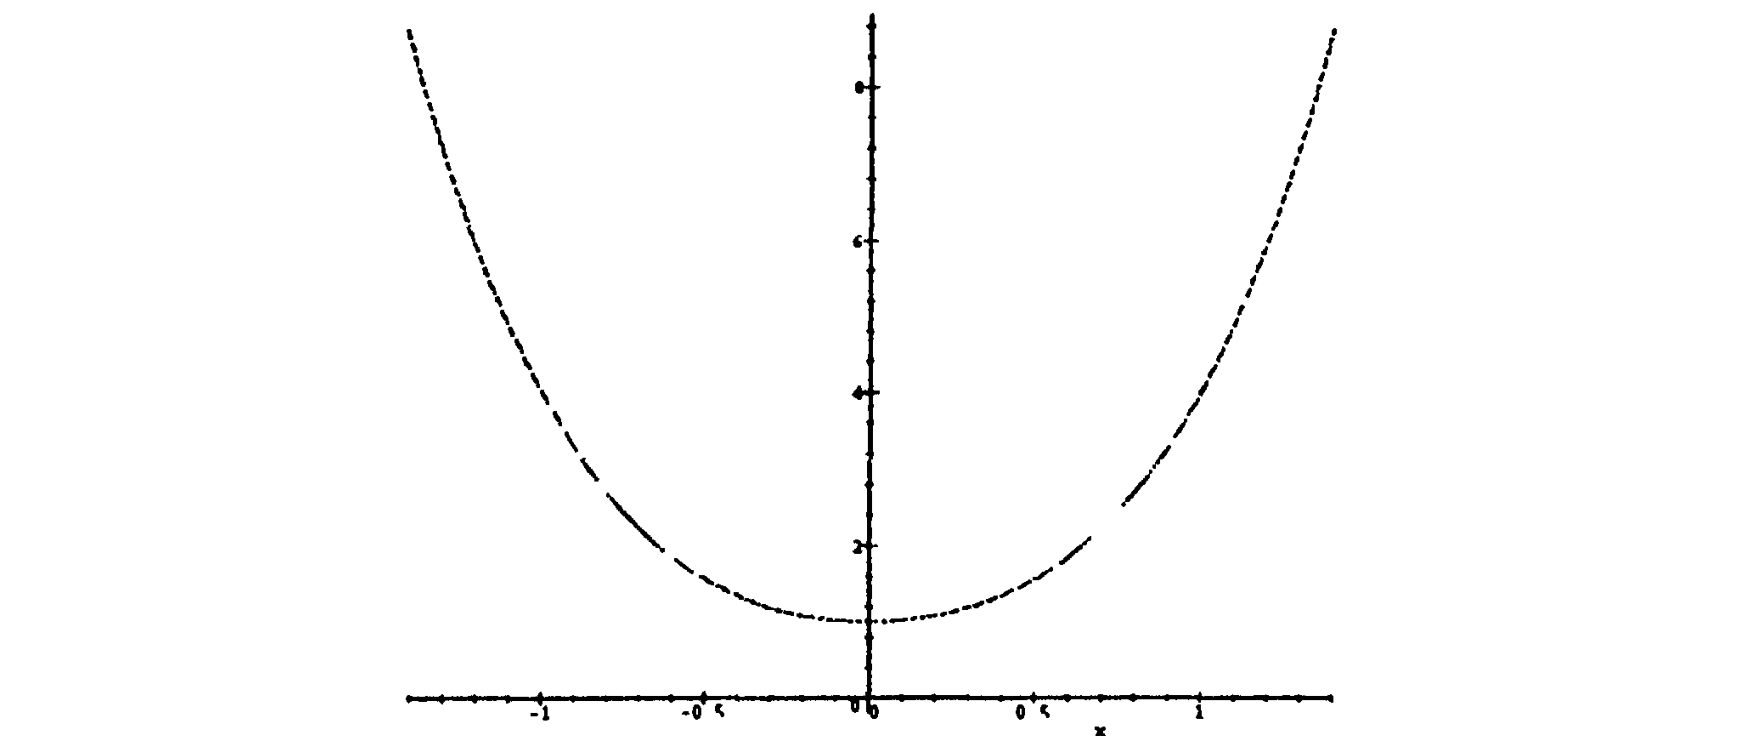
\includegraphics[width=0.72\textwidth]{figs/fig_p031_1.png}
  \caption{$v^2>0$ 时的势能曲线：曲线在原点有唯一极小，横轴为场 $\phi$（图中标为 $x$），纵轴为势能 $V$。（原文 Figure 1，p.31）}
  \label{fig:p31-1}
\end{figure}

\textbf{情形 1（Case 1）}：$v^2>0$。此时能量的极小在 $\phi=0$ 处达到。先考虑规范耦合为零的情形：$e^2=0$。此时我们的理论是纯（自由）阿贝尔规范场论与 $\phi^4$ 理论的直积。因此它有唯一的真空，而出现在谱的下部的粒子是一个无质量矢量，即规范玻色子（gauge boson，来自规范场论），以及两个有质量的实标量（来自 $\phi^4$ 理论）。

若我们把 $e^2$ 取为小的非零值，情况应保持不变。的确，有质量的标量肯定不会发生任何变化（Hilbert 空间中由带非零电荷的态——如这些标量——所构成的子空间在最低阶近似下有质量间隙（mass gap），而"有质量"是一个开条件（open condition））；此外，它们的质量必须相等，因为无穷远处存在一个 $U(1)$ 对称性（即常值 $\varepsilon$ 对应的 $Q(\varepsilon)$），它禁止质量不等。$Q(\varepsilon)\neq0$ 这一点是清楚的，因为在 $e^2=0$ 时就是如此，而此时 $Q(\varepsilon)$ 表示的正是 $U(1)$ 整体对称性。当 $\varepsilon$ 取单位切向量时，算符 $Q(\varepsilon)$ 称为电荷算符（operator of electric charge）。

此外，无质量矢量不可能变成有质量的。的确，回忆一下：无质量矢量意味着 $SO(3,1)$ 的一个不可约表示，其 $p^2=0$、自旋为 $1$，亦即光锥（light cone）上一个二维等变向量丛（equivariant vector bundle）的截面空间。这个向量丛不可能形变为双曲面（hyperboloid）上的等变向量丛，

% ===== 原文 p.32 =====
因为双曲面（hyperboloid）上一点的稳定化子群 $SO(3)$ 没有二维不可约表示。因此，小耦合下的量子理论将具有同样的粒子——两个有质量标量（$\phi$ 的实部与虚部）和一个无质量矢量（规范玻色子）。

% [Tutor Note: 这段"不可形变"论证的表示论内核值得点明：$p^2=0$ 时的小群（little group）是 $ISO(2)$，无质量自旋 1 的二维自由度来自其转动子群 $SO(2)$；而 $p^2=m^2>0$（"双曲面"即质量壳）时小群是 $SO(3)$，有质量自旋 1 需要三维表示。作者以"$SO(3)$ 没有二维不可约表示"来表述"不能连续形变"，本质上是说无质量矢量要获得质量必须多出一个纵向自由度，而该自由度只能来自别处（在 Higgs 机制中正来自标量）。此处 $SO(3,1)$ 的等变丛语言是把表示论陈述翻译成拓扑陈述，注意"光锥上二维"与"双曲面上三维"的维数差正是纵向自由度。]

\textbf{评注（Remark）}。上述关于无质量矢量不可形变的论证在二维或三维中失效。例如在三维中，无质量矢量恰好是锥上的函数空间，而它可以成功地形变为双曲面上的函数空间。当人们在纯 $U(1)$ 规范场论中引入 Chern–Simons 项 $c\int A\wedge dA$ 时，这确实会发生。理论仍保持自由，但变成有质量的，给出一个有质量标量。在我们所考虑的理论中（就三维而言），这不可能动力学地发生，因为 Chern–Simons 项在改变定向时变号；但在别的理论中这可以发生。

事实上，在量子理论中算符 $Q(\varepsilon)$（对 $\varepsilon$ 作适当归一化后）具有整特征值，因而（在量子理论中）定义了相应 Hilbert 空间的 $\mathbb{Z}$-分次（$\mathbb{Z}$-grading）。特别地，由于 $Q(\varepsilon)\neq0$，而 $Q(\varepsilon)$ 与一切局域算符对易，Hilbert 空间存在一些扇区（即 $Q(\varepsilon)$ 非零的那些扇区），它们不能通过作用局域算符从真空到达。这表明我们根本性地违反了 Wightman 公理：算符代数在物理 Hilbert 空间中的表示不是不可约的。然而，理论仍然只有一个真空：$Q(\varepsilon)$ 非零的扇区中的最低能量为正。

\begin{figure}[htbp]
  \centering
  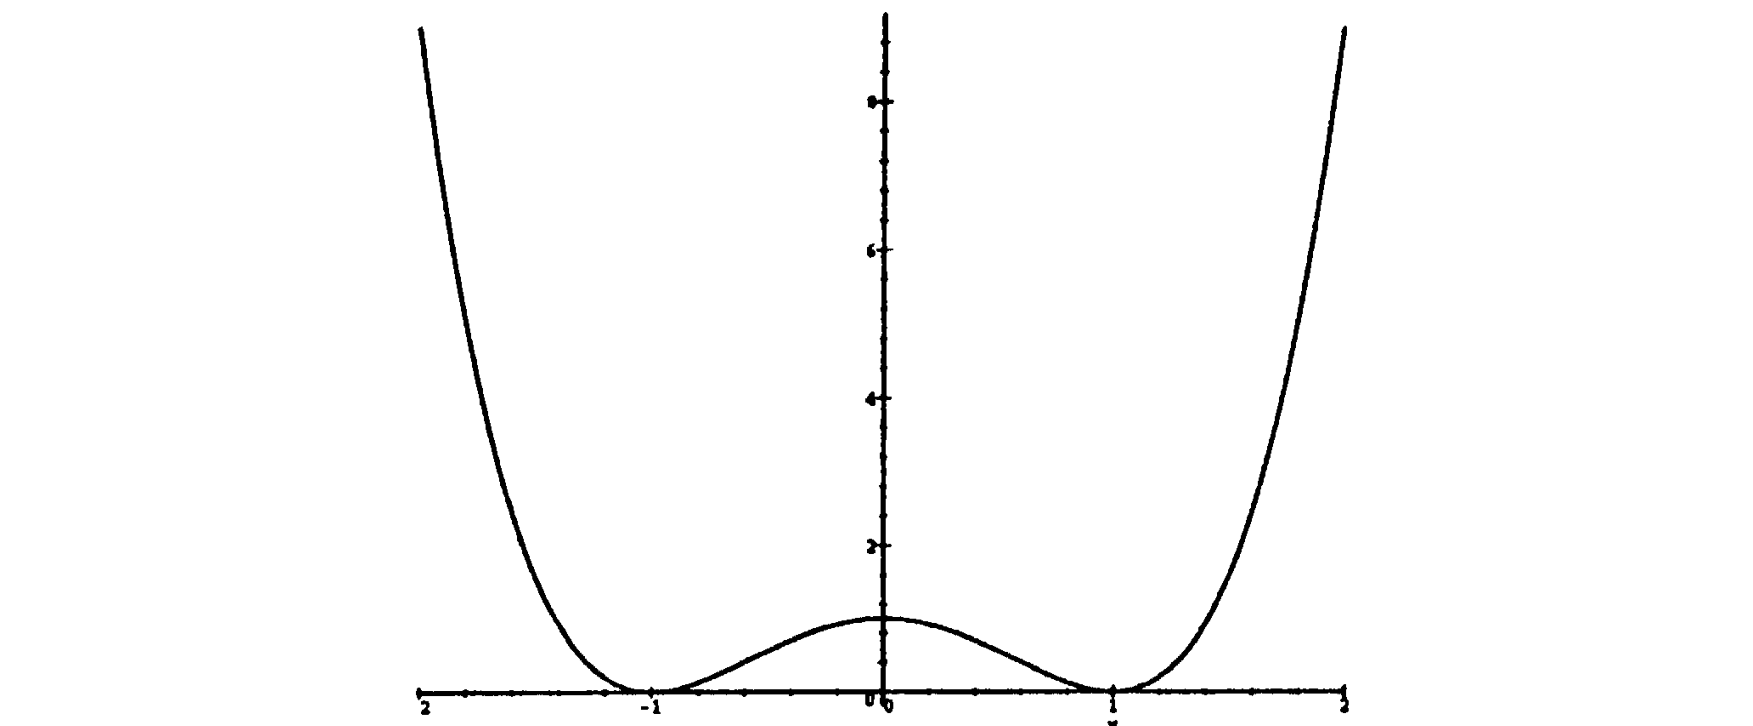
\includegraphics[width=0.72\textwidth]{figs/fig_p032_1.png}
  \caption{$v^2<0$ 时的势能曲线（"墨西哥帽"的截面）：两个简并极小位于 $|\phi|=b$ 处，横轴为场 $\phi$ 的实部（图中标为 $x$），纵轴为势能 $V$。（原文 Figure 2，p.32）}
  \label{fig:p32-1}
\end{figure}

\textbf{情形 2（Case 2）}：$v^2<0$。令 $v^2=-b^2$。那么经典上能量的极小在圆 $|\phi|=b$ 上达到。这意味着任何有限能量位形在无穷远处都具有性质 $\phi=be^{i\theta_0}$，其中 $\theta_0$ 是常数。因此，通过一个在无穷远处有有限极限的规范变换，我们可以安排 $\phi$ 为实且为正：$\phi=b+w$，其中 $w$ 是新的实变量。用这些新变量写出拉氏量，我们将得到如下形式的二次部分：

\begin{equation}
  \tag{2.4}
  \label{eq:2-4}
  L_{\text{quadratic}}=\frac{1}{4e^2}\int F^2+\int d^4x\left((dw)^2+M^2w^2\right)+\int d^4x\,b^2A^2.
\end{equation}

% [Tutor Note: 由 (2.4) 可以反推作者对协变导数的约定。$|D_A\phi|^2$ 在 $\phi=b$ 处给出规范场质量项：若用通常的 $D_A=\partial+ieA$，该项应为 $e^2b^2A^2$，而 (2.4) 中系数恰为 $b^2$，说明作者把电荷 $e$ 吸收进了 $A$（即 $D_A=\partial+A$），或者此处为示意性写法。读质量谱时必须先把 $A$ 归一到标准动能项 $\frac{1}{4}F^2$（即 $A\to eA$），此时 $A^2$ 系数变为 $e^2b^2$，与 $\frac{1}{4}F^2+\frac12m_A^2A^2$ 相比得 $m_A^2=2e^2b^2$。同理，$M^2$ 与 $\lambda b^2$ 同阶：把 $\frac{\lambda}{8}(|\phi|^2-b^2)^2$ 在 $\phi=b+w$ 处展开得 $\frac{\lambda}{2}b^2w^2$，与 (2.4) 中 $M^2w^2$ 对照即可定出 $M^2$。]

由 (2.4) 可见，现在所有场都是有质量的。当然，拉氏量 (2.4) 对 $A$ 不再规范不变，因为我们已经把规范对称性"用掉"以使得 $\phi$ 为实。

因此，对于小的耦合值，相应量子理论的红外极限是平凡的。特别地，不存在无质量规范玻色子：它们

% ===== 原文 p.33 =====
已被 $\phi$ 场"吃掉"（eaten）。这种情形称为 Higgs 现象（Higgs phenomenon），或规范对称性的自发破缺。

注意，尽管存在看起来像零能量态圆圈的东西，我们的理论仍然只有一个真空。换句话说，圆上所有的点被视为同一个态，理由是它们彼此规范等价，因而定义等价的实现（即给出相同的规范不变局域算符的期望值）。这是规范对称性破缺与整体对称性破缺之间的根本区别。在整体对称性破缺中，圆上的点代表理论的不同真空（不同实现），因为存在非对称的算符，它们在该圆的不同点上取不同的期望值。

总结起来，「规范对称性破缺」一语主要指 Higgs 机制，即 Higgs 现象：在诸如 $v^2<0$ 这样的模型中，规范场尽管耦合很弱也获得质量。在严格得多的条件下（见第 10 讲），人们可以对"Higgs 相"的含义给出公理化的解释。但就这个术语最常用的意义而言，「Higgs 机制」不过是即便耦合很弱也能得到有质量谱（或至少使无质量自旋 1 场的数目小于规范群维数）的一条途径。它之所以重要，是因为它是规范场论所能做的最简单的事情之一，而且它在自然界中出现在弱相互作用里。

\textbf{评注（Remark）}。若有人试图用公式 (2.3) 计算情形 2（对称性破缺时）的 $Q(\varepsilon)$，答案将是零，因为被积函数在无穷远处迅速衰减。当 Higgs 机制发生时，与规范对称性相联系的守恒荷为零。

% [Tutor Note: "荷为零"与 (2.3) 的边界积分一致：在 Higgs 相中 $F$ 以 $e^{-m_Ar}$ 指数衰减（$m_A$ 为规范玻色子质量），故 $r\to\infty$ 时球面积分趋于零，$G_\infty$ 的生成元在真空上实现为零。这与电动力学中"总电荷由无穷远 Gauss 通量给出"完全一致：场被屏蔽后通量为零。反过来，情形 1 中 $F\sim Q/r^{2}$ 衰减恰好使 (2.3) 给出非零常数，这正是电荷算符的边界定义。]

在情形 2 下于红外中出现的粒子，按照 (2.4)，是一个有质量矢量（$A$）和一个有质量标量（$\phi$）。只有一个标量，因为 $\phi$ 现在是实的。因此，在表示论的层面上，情形 2 中出现的 Higgs 现象归结为 Poincaré 群表示的一种形变：无质量矢量加无质量标量形变为一个有质量矢量。作为对照，回忆一下：单独一个无质量矢量不能形变为有质量表示。

最后，考虑特殊情形 $v^2=0$。此时经典上我们与 $v^2>0$ 时一样没有对称性破缺，粒子是一个无质量矢量和两个无质量标量。然而，这不应是量子答案，因为此位形在微扰下不稳定。

% [Tutor Note: 作者说 $v^2=0$ 的位形"在微扰下不稳定"，略去了依据。其一是树级势 $\frac{\lambda}{8}|\phi|^4$ 在原点处二阶导数为零，$\phi=0$ 只是高阶临界点，任何微小扰动（包括圈修正）都会移动真空；其二是量子修正会生成 Coleman–Weinberg 型有效势，其中规范场圈给出 $\sim e^4|\phi|^4\ln(|\phi|^2/\mu^2)$ 的项，使原点变成极大值、真空移到 $\langle|\phi|\rangle\neq0$ 处（即量纲穿越，dimensional transmutation）。参见 Sidney Coleman 与 Eric Weinberg, Phys. Rev. D7 (1973) 1888。]

\textbf{评注（Remark）}。如果我们出发的拉氏量不是红外地自由的（IR free），比如说它是某个渐近自由（asymptotically free）规范场论的拉氏量，那么上面讨论的经典分析在量子理论中不适用。此时理论的红外行为一般难以确定。各种事情都可能发生，其中一些我们将在本学期我后续的讲课或 Seiberg 的讲课中听到。除其他可能性外，人们可以以远比 Higgs 机制更奇特、更难理解的方式得到有质量谱；或者人们可以在红外中生成一个并非原经典规范对称性子群的未破缺规范对称性。

% ===== 原文 p.34 =====
% 原文 §2.3
\subsection{对称性破缺与规范化}

最后，让我们讨论整体对称性破缺与规范对称性破缺之间的联系。设我们有一个场论的拉氏量 $L$（譬如在四维中），它具有整体 $U(1)$ 对称性。一个典型的例子是：理论包含一些标量场 $\phi_j$，它们是 Hermite 向量丛的截面，而 $U(1)$ 通过这些截面的乘法 $e^{in_j\theta}$ 作用。通过引入 $U(1)$ 规范场 $A$ 与新的拉氏量，这个 $U(1)$ 对称性可以被规范化（gauged）：

\begin{equation}
  \tag{2.5}
  \label{eq:2-5}
  L_{\text{gauged}}=\frac{1}{4e^2}\int F_A\wedge *F_A+L_A,
\end{equation}

其中 $L_A$ 由原来的物质拉氏量 $L$ 把 $\phi_j$ 的所有导数替换为协变导数（covariant derivative）而得到。

% [Tutor Note: 电荷 $n_j$ 必须是整数，$e^{in_j\theta}$ 才在 $\theta\to\theta+2\pi$ 下良定义，这也保证了 (2.5) 中 $F_A\wedge *F_A$ 的 $1/4e^2$ 归一化在 $U(1)$ 丛的整系数下自洽。另注意 $L$ 与 $L_{\text{gauged}}$ 都不是拉氏量密度而是作用量（同 p.31 的 $\mathcal{L}$），故 $L_A$ 中"替换导数"应理解为对整个作用量中的 $\partial_\mu\phi_j\to D_\mu\phi_j=(\partial_\mu+in_jA_\mu)\phi_j$。]

上述论断是：若 $L$ 是红外地自由的，则在三维以上、小规范耦合下，由 $L$ 与 $L_{\text{gauged}}$ 所定义的两个理论的对称性破缺行为相同。（在二维或三维中讨论需要一些修改，原因是 $U(1)$ 规范场论中的"禁闭"（confinement），我们将在本学期稍后研究它；此外还有某些其他原因，将在今天稍后以及以后的讲课中讨论。）也就是说，若 $L$ 有整体对称性破缺，则 $L_{\text{gauged}}$ 有 Higgs 机制；反之亦然。

的确，让我们考虑两种情形。

\textbf{情形 1（Case 1）}：无整体对称性破缺。我们假定理论足够一般（generic），使得没有无质量带电标量。（这在我们上面的例子中相当于避开临界情形 $v=0$。）在 $e$ 小的极限下，Hilbert 空间是量子化 $L$ 所得的 Hilbert 空间 $\mathcal{H}_L$ 与一个自由无质量自旋 1 场的 Hilbert 空间 $\mathcal{H}'$ 的张量积。$U(1)$ 非平凡地作用，其作用实现于 $\mathcal{H}_L$ 上。在缺少带电无质量标量的情况下，这个含一个无质量自旋 1 场的谱是稳定的；对足够弱的耦合，它不会发生任何变化。

\textbf{情形 2（Case 2）}：整体对称性破缺。此时在能量的极小处，带电场 $\phi_j$ 不为零。不存在不变的经典基态，并且存在一个与这个对称性破缺相应的 Goldstone 玻色子。在此情形下，取一个真空态以及一个在该真空中不为零的分量 $\phi_j^{(n)}$。在规范化的理论中，我们可以作一个规范变换，使这个分量为实且为正。这表明：若不存在其他无质量粒子（特别地，没有其他破缺的整体对称性），则理论中所有的场都将变成有质量的。于是我们得到规范对称性的破缺。在描述这一情形时，我们使用了经典语言，假定了 $L$ 弱耦合；但这一讨论可以抽象地进行，只需假定 $L$ 所描述的理论中 $U(1)$ 对称性是自发破缺的。

这些考虑只在规范耦合小时成立。（若我们在四维取非阿贝尔规范群，那么在情形 1 中还有进一步的限制：只有当 $\beta$ 函数为正、从而规范耦合在红外流向零时，这一分析才适用。）

% 原文 §2.4
\subsection{不存在更高自旋的无质量粒子}

现在我们对四维的红外地自由理论作一般的考察。（以下的考虑可推广到四维以上，但在四维以下会变得平凡……）

% 说明：本句在原文 p.1153 续完（"… below four dimensions"），其内容属于第二部分（p.35 起）。
